\chapter{Implementation}
\label{cha:implementation}
In this chapter, the implementation of a prototype of the system is presented. Due to time constraints and the overall complexity of the system, some features that are presented in Chapter \ref{cha:design} are not implemented in the final prototype. They mostly consist of individual classifiers to enrich user data such as marital status or number of children, which ultimately do not impact the larger structure and functionality of the system. In fact, this can be seen as proof that the system design meets the requirement of being highly customizable and expandable.

The whole prototype is developed in Python, one of the most complete programming languages when it comes to the availability of machine learning and other user-made libraries. Every component presented in the design section consists in a separate package. In the sections below, those components are described in more detail one by one: the implementation choices for the database and the pub/sub system; how data is collected only from Twitter due to privacy reasons; how the enrichments are performed and what kind of external tools are used for that purpose; what clustering algorithm is used and why; what tools are used to assign an identity to personas; and how the web API was implemented and what functionalities in particular it provides. Finally, a section is dedicated to showing the typical flow of actions and data through the system, in order to understand how all components interact with each other.

\section{Database}
Given the unstructured nature of the data that the system handles, a non-relational database was chosen. In particular, the choice fell on \texttt{Redis}\footnote{\url{www.redis.io}}, an open source, in-memory data structure store that can be used both as a database, cache and message broker. By working in-memory, it can achieve high performance over traditional databases. Data is stored in key/value pairs, as in a typical dictionary data structure: keys are always strings, while values can be a range of supported data types. For our use-case, since complex, nested data models need to be stored, we installed \texttt{RedisJSON}\footnote{\url{www.redislabs.com/blog/redis-as-a-json-store}}, a module that adds support for a JSON data type. This means that all models are converted to and from JSON every time they need to be stored or retrieved from the database. The database runs in a dedicated Docker container.

\section{Pub/Sub}
The Pub/Sub queue system is implemented with the MQTT protocol. The implementation provided in the library \texttt{paho-mqtt}\footnote{\url{www.eclipse.org/paho/}} is used. All the messages are sent and received with a \emph{Quality of Service} (QoS) level of 1, which guarantees that every message is delivered at least once. This allows for the modules that disconnect for any reason to recover all not-received messages once they go back online.

\section{Data collection}
\label{sec:data_collection_imp}
The data source on which the prototype is based is Twitter. Facebook products (such as Facebook itself and Instagram) were considered, but developing an application that works with them has become difficult due to strict privacy policies. In fact, in order to collect data of a user through their API, it is first needed to get explicit authorization of the user. Finding enough users available to share their data for the development of this system would have been a lengthy process. Also other services were taken into consideration, but were ultimately scrapped due to a lack of an API or the unavailability of a free version of the latter.

In order to use the Twitter API, it is first needed to submit a request explaining what you are going to use the API and the collected data for. After confirmation, the API provides a free plan, although with some restrictions on the rate at which requests are made (e.g. 1500 requests every 15 minutes to retrieve tweets). The free plan allows us to get all the information that is needed: user profile information and user tweets. The API is accessed using the \texttt{tweepy}\footnote{\url{www.tweepy.org}} library, which provides a convenience class that handles requests and parameters. It also handles rate limitations by suspending the process until a new time slot is available.

\section{Data enrichment}
This component is divided in two smaller modules that are run independently: one to enrich activities, and one to enrich data sources. They are presented in the sections below.

\subsection{Activity enrichment}
The main task of this module is to extract \emph{language}, \emph{sentiment} and \emph{entities} from an activity, which can contain text and/or images.

An \emph{entity} is a person, an object or a concept that has an article on Wikipedia; for example, the phrase \textit{"I'm studying computer science at the university"} has two entities - \texttt{Computer science} and \texttt{University}. Entity extraction is a powerful approach to figure out what a user talks about in an activity: it supports both texts and images, and it is expandable to many languages (it is only needed, for example, to convert entities, which are Wikipedia articles, to their English article counterpart).

While there exist tools that allow entity extraction from images, such as the \texttt{Cloud Vision API} of Google Cloud\footnote{\url{cloud.google.com/vision}}, they were not used in the prototype due to their heavily restricted free plans. This limits the prototype to only work with texts, but, in a production environment, support for images could greatly improve the accuracy of the final results, since many social media posts don't include any text.

For all three enrichments, we used an external semantic analyzer called \texttt{Dandelion}\footnote{\url{dandelion.eu}}, developed by Spazio Dati\footnote{\url{spaziodati.eu/it}}. It works by using Wikipedia pages as entities, as explained in Section \ref{subsubsec:activity_enrichment}. It provides useful options to optimize entity extraction from short texts coming from social networks, which makes it adequate for our use-case. Additionally, it supports a total of 50 languages, 43 of which are in beta support. The free plan allows the use of 1000 credits per day, and 2.1 credits are used for enriching each activity. This means that only 476 activities can be enriched per day for free. U-Hopper provided a token with 10000 credits, which allows to enrich ten times that amount.

\subsection{Data source enrichment}
This module has the task of enriching the \texttt{Attributes} properties detailed in Section \ref{subsubsec:user_profile_enrichment}.

\textbf{Gender}, \textbf{age} and \textbf{type} are predicted based on the profile image of a user on a given data source. A customized version of the \texttt{M3-Inference}\footnote{\url{github.com/euagendas/m3inference}} library is used for this purpose. Since predicting an exact age is too difficult, four age brackets are given as possible output: $\leq$18, 19-29, 30-39, $\geq$40. In case a profile image is not available, an external API called \texttt{NamSor}\footnote{\url{www.namsor.com}} is used to predict gender and type from a first or full name. This is not always reliable, since the name field is free form on Twitter, which means that a user can choose a fictional name (as opposed to Facebook, which enforces the use of real names).

The \textbf{preferred language} is chosen by keeping a map between all the languages the user has used in their activities, and how many times each language is used. The preferred language is therefore the most used language throughout all activities.

\textbf{Attitude} is simply computed as the average of all sentiment scores found in the user's activities, while \textbf{interests} are more complex to extract. First, the system keeps track of an \emph{entity map} for each data source; it consists in a dictionary where the keys are the entities found in the user's activities, and the values are how many times that entity was found. This is then given as input to a Tapoi model, proprietary of U-Hopper, which functions as follows:
\begin{enumerate}
    \item the model is defined by a fixed set of categories of interest, which represent the full set of interests that are expected as output. Those categories are represented by Wikipedia pages, and in our case are the following: \texttt{Arts, Filmmaking, Cooking, Culture, Economy, Entertainment, Fashion, Geography, Health, History, Literature, Music, Nature, Philosophy, Po\-li\-tics, Religion, Science, Sports, Technology};
    \item the model traverses the Wikipedia graph upwards, starting from each entity found in the entity map, for a fixed number of steps (usually 5);
    \item each time a category of interest is found while traversing the graph, a score is added to that category, proportional to the number of times the respective entity is found in the entity map;
    \item the output is a mapping between each category of interest and their respective scores, which are in the $[0,1]$ range. All scores sum up to 1, and a high score means that the user is interested in the corresponding category.
\end{enumerate}

Two Tapoi models were made available by U-Hopper for this thesis: one that works on English Wikipedia, and one on Italian Wikipedia. While it is possible to use both models for analyzing English and Italian activities, this would mean supporting only two languages. The implemented solution, instead, only uses the English model: if an entity is in another language, it first gets converted to the respective English page on Wikipedia (when available) through the MediaWiki API\footnote{\url{www.mediawiki.org/wiki/API:Main_page}}. The English model was chosen over the Italian one due to English Wikipedia having the largest number of articles than any other language.

As for the rest of the \texttt{Attributes}, they are not implemented due to time constraints, but other Tapoi models exist to predict many of them.

\section{Clustering}
The most important implementation choices for this component are: the features on which to perform clustering; the choice of a distance metric, needed to compute how similar (or dissimilar) two users are; and the actual clustering algorithm. The order in which those implementation choices are listed is not casual: the choice of algorithm depends on the distance metric, and the distance metric depends on what types of features are used.

\subsection{Features}
The chosen features are the \texttt{Attributes} properties that are implemented, minus the type; that is: gender, age, preferred language, attitude and interests. The type is excluded because we decided to deal only with users who are classified as "humans", since personas are ultimately fictional individuals. The features are a mix of \emph{nominal}, \emph{ordinal} and \emph{numerical} data:
\begin{itemize}
    \item nominal data is data that takes on discrete values and does not possess a meaningful order. In our case, gender and preferred language fall under this category;
    \item ordinal data is data that takes on discrete values but possesses a meaningful order. Age is an example of this: it can take on three different values ($\leq$18, 19-29, 30-39, $\geq$40), and it makes sense to say that the bracket $\leq$18 is closer to 19-29 than it is to 30-39;
    \item numerical data is data that takes on continuous values. Attitude is an example, as it is a decimal number in the range $[0,1]$.
\end{itemize}
Interests do not fall directly into any category, but are closer to a mix of nominal data (interest labels) and numerical data (scores).

\subsection{Distance metric}
\label{subsec:distance_metric}
Since we are dealing with mixed data, the most commonly used distance metric, euclidean distance, cannot be used, as it only works with numerical data. This also locks out the choice of K-Means as the clustering algorithm, since it relies on the concept of mean, which is only meaningful in a continuous space. The chosen distance metric is therefore the \emph{Gower distance}, which supports mixed data~\cite{tuerhong2014gower}. It is defined as follows:
\begin{equation*}
    D_{Gower}(x_1,x_2)=\frac{1}{p}\sum_{j=1}^{p}d_j(x_{1j},x_{2j})
\end{equation*}

In words, it is computed as the average of partial dissimilarities across objects with $p$ features. A partial dissimilarity $d_j$ is computed between two objects $x_1$ and $x_2$ on a particular feature $j$, and depends on the type of the feature (ordinal, numerical or nominal):
\begin{equation*}
    \begin{split}
        d_{j,ord}(x_1,x_2)=\frac{\lvert rank(x_{1j})-rank(x_{2j})\rvert}{range_j}
    \end{split}
    \qquad
    \begin{split}
        d_{j,num}(x_1,x_2)=\frac{\lvert x_{1j}-x_{2j}\rvert}{range_j}
    \end{split}
    \end{equation*}
    \begin{equation*}
        d_{j,nom}(x_1,x_2)=
        \begin{cases}
            1 & \text{if}\ x_{1j}\neq x_{2j} \\
            0 & \text{otherwise}
        \end{cases}
\end{equation*}
where $rank(x_j)$ is the ordinal number assigned to feature $x_j$, and $range(j)$ is defined as the difference between the maximum and minimum values of feature $j$.

A modified version of the Gower distance is used in our system: instead of simply averaging all partial dissimilarities, a weighted average is computed. This allows to give more weight to features that can be considered more important, like the interests in our case.

\subsection{Clustering algorithm}
Since we have defined a custom distance metric, only algorithms that support either a distance function as a parameter or a precomputed distance matrix can be chosen. Given $n$ users, we define a distance matrix $M[n\times n]$, where each cell $M[i,j]$ contains the distance between user $i$ and user $j$.

The chosen algorithm is called \emph{K-Medoids}\footnote{\url{en.wikipedia.org/wiki/K-medoids}}, an alternative version of K-Means that accepts a precomputed distance matrix as an input parameter. Instead of computing a centroid as the mean of all objects in a cluster, the algorithm chooses a medoid; it can be defined as the object of a cluster whose average dissimilarity to all the other objects of the cluster is minimal, that is, the most centrally located point in the cluster. Using K-Medoids also has the advantage that medoids, as opposed to centroids, are real data points (i.e. users), which means that they can be directly given as input to the persona generation component.

The main challenge remains deciding the right number $k$ of clusters, which needs to be specified a priori. The chosen way is trying models with different values of $k$, ranging from 2 to 10, since we do not want a large number of clusters. For each model, we compute the average \emph{silhuette score}\footnote{\url{en.wikipedia.org/wiki/Silhouette_(clustering)}}: it is a number between -1 and 1 which measures how similar an object is to its own cluster (cohesion) compared to other clusters (separation). The optimal number of clusters is therefore the one that maximizes the average silhuette score.

\section{Persona generation}
This component is simpler than the others, especially since the clustering algorithm outputs representative users with meaningful attributes. Given a representative user, it is needed to enrich it with a name, photo and textual description.

The \textbf{name} is generated through an external API called \texttt{Name Parser}\footnote{\url{parser.name}}. It allows to optionally specify a gender and a country, in order to get demographically accurate names.

The \textbf{photo} is taken from a predefined set of photos; for the purpose of the prototype, the set is composed of five photos for each gender and age bracket, for a total of 40 photos. The photos were taken manually through a website\footnote{\url{thispersondoesnotexist.com}} that uses AI to generate pictures of people that do not exist.

The \textbf{description} was not implemented due to time constraints, but a valid approach would be to write one or more templates that can be appropriately filled with the persona attributes.

\section{Web API}
The web API is implemented using the \texttt{Flask}\footnote{\url{flask.palletsprojects.com/en/2.0.x/}} framework, extended with the \texttt{Flask-RESTful} library. The chosen method for managing authentication and authorization is a JWT Token, a particular implementation of token/bearer authentication. Each token contains the ID number of the account that generated the token, and it is checked in order to grant or deny access to a requested resource. It also contains an expiration date, after which the token is no longer valid. In the prototype, like is often seen in web APIs, the expiration date is not set; this means that it is up to the user of the service to keep the token secret. In any case, it is possible to regenerate a token, a process which invalidates the previous one.

Figure \ref{fig:api_funcs} shows the main functionalities provided by the web API (the lock icons show what resources need authorization). The complete specification and documentation is available at the link below:
\begin{center}
\url{app.swaggerhub.com/apis-docs/nicola-farina/personas/1.0.0}
\end{center}

\begin{figure}[h]
\centering
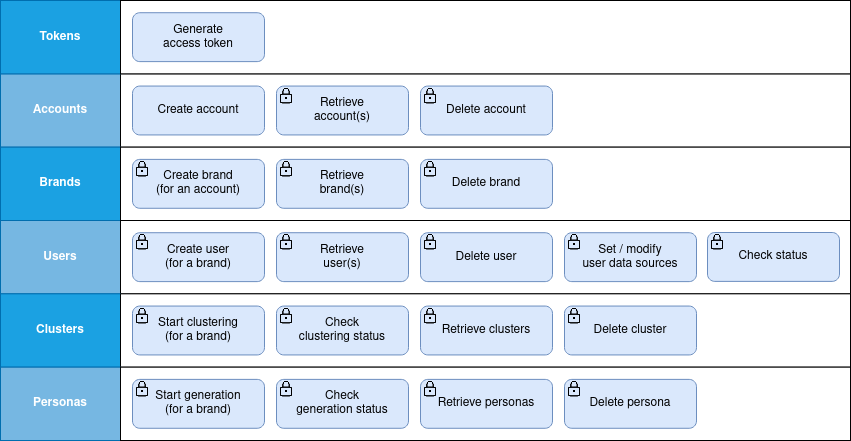
\includegraphics[width=1\textwidth]{img/APIfuncs.png}
\caption{Functionalities provided by the API}
\label{fig:api_funcs}
\end{figure}

\section{Flow of the system}
Figure \ref{fig:enrichment_flow} shows a typical flow of the data collection and enrichment components in detail, while Figure \ref{fig:flow} shows the flow of the whole system. 

The implementation of the collection and enrichment components takes the advantages of real time data processing while still allowing to keep track of progress. In order to do so, a \texttt{Computation} object is created whenever a process of data collection and enrichment begins: it is simply composed by a unique ID and a \emph{status} field. Those objects are stored in the database, and every 24 hours all computation objects whose value equals \emph{done} are deleted, since they are no longer needed. Another advantage of keeping track of the progress is that data sources can be sent for enrichment only when all related activities are enriched. This is preferable because, if there was no way to keep track of how many activities have been enriched, data sources would have to be enriched after every single activity. This would result in a lot of external API calls, which may have severe rate limitations.

\begin{figure}[h!]
\centering
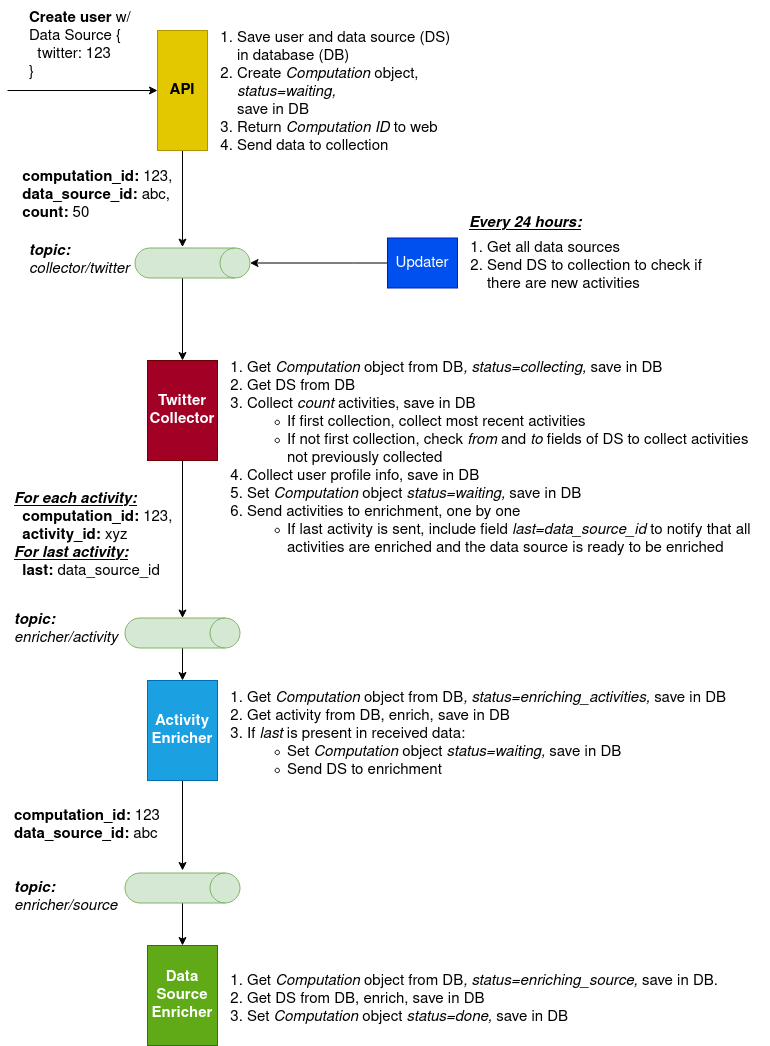
\includegraphics[width=0.95\textwidth]{img/EnrichmentFlow.png}
\caption{Detailed flow of collection and enrichment components}
\label{fig:enrichment_flow}
\end{figure}

\begin{figure}
\centering
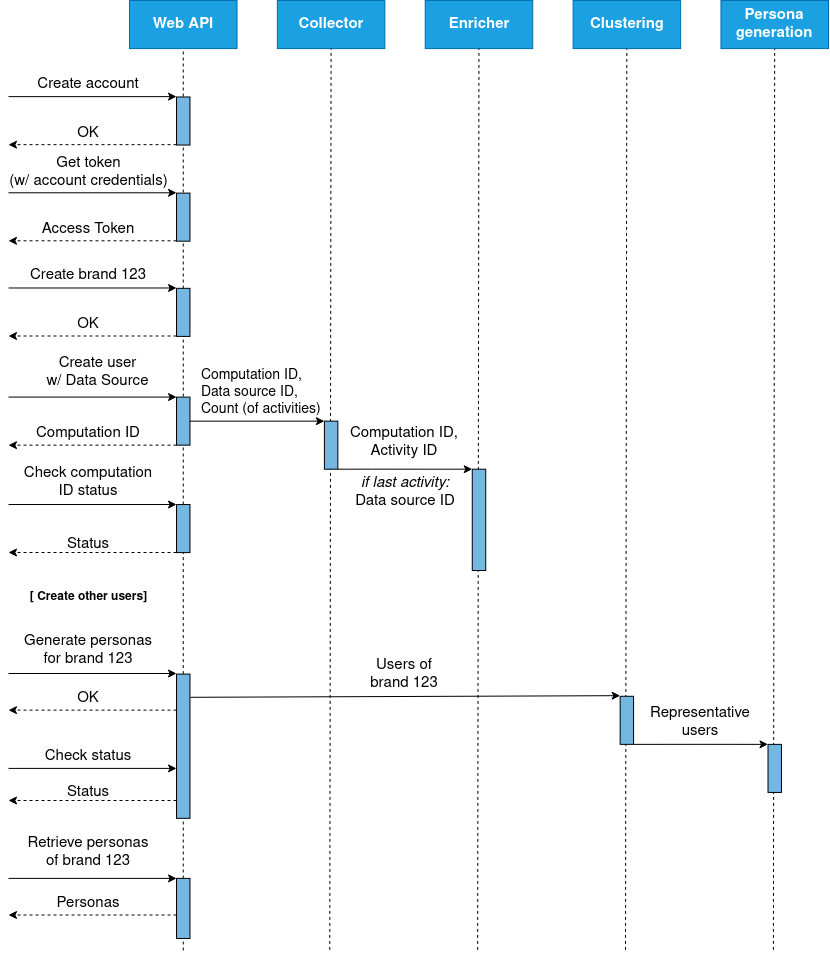
\includegraphics[width=\textwidth]{img/SystemFlow.png}
\caption{Typical flow of actions and data in the system}
\label{fig:flow}
\end{figure}
